\documentclass[stu, 10pt, floatsintext]{apa7}

% Establecer el idioma en español
\usepackage[spanish]{babel}
\usepackage{apacite}
\usepackage[utf8]{inputenc}
\usepackage{graphicx}
\usepackage{float}
\usepackage[normalem]{ulem}
\usepackage{hyperref}
\definecolor{colorEnlace}{RGB}{0, 0, 0}
\hypersetup{
	colorlinks=true,
	linkcolor=colorEnlace,
	citecolor=colorEnlace,
	urlcolor=colorEnlace,
	pdfauthor={Davis Bremdow Salazar Roa},
	pdftitle={Circuitos Lineales con Amplificadores Operacionales}
}


%opening
\title{Memoria ROM}
\author{Davis Bremdow Salazar Roa}


% 
\usepackage[spanish]{babel}
\usepackage{float}
\begin{document}
	\renewcommand{\baselinestretch}{1.3}
	\thispagestyle{empty}
	
	\begin{center}
		\LARGE \textbf{UNIVERSIDAD NACIONAL DE SAN ANTONIO ABAD DEL CUSCO}
		
		\Large \textbf{FACULTAD DE INGENIERÍA ELÉCTRICA, ELECTRÓNICA, INFORMÁTICA Y MECÁNICA}
		
		\Large \textbf{ESCUELA PROFESIONAL DE INGENIERÍA ELECTRÓNICA}
		
		\vspace{5mm}
		
		
\includegraphics[width=0.3\textwidth]{logo2C.png}
		
		%\Large \textbf{INFORME PREVIO EXPERIENCIA N°3}
		
		\rule{\textwidth}{1pt} % Línea superior
		
		\vspace{10pt} % Espacio entre líneas
		
		\Large \textbf{LABORATORIO N°7}
		
		\vspace{2pt} % Espacio entre líneas
		
		\rule{\textwidth}{1pt} % Línea inferior
		
	\end{center}
	
	\renewcommand{\baselinestretch}{1.5}
	
	
	\large \textbf{Curso:} Laboratorio de sistemas digitales II
	
	\large \textbf{Docente:} Ing. Palomino Peña Celso
	
	\large \textbf{Semestre:} 2024-I
	
	\large \textbf{Alumnos:}
	
	\begin{center}
		\begin{tabular}{@{}l @{\hspace{4cm}} l @{\hspace{2cm}} r@{}}
			Lujan Edilia Huamanga Chumbes & & 201250 \\
			Jesus Leonardo Ima Chuquichampi & & 200834 \\
			Bremdow Salazar Roa & & 200353 \\
			Aaron Coyla Quispe & & 200832 \\
		\end{tabular}
	\end{center}
	
	
	\vfill %Esto estará en la parte inferior de la página
	
	\begin{center}
		%Cusco - Perú
		
		2024
	\end{center}
	
	% Inicia una nueva página
	\newpage
	
	% Establece el justificado izquierdo para el texto
	%\raggedright
	
	% Establece la sangría de cada nuevo párrafo en 1.27 cm
	\setlength{\parindent}{1.27cm}
	
	% Ajusta el espaciado entre líneas a 2 (espaciado doble)
	\renewcommand{\baselinestretch}{2}
	
	\renewcommand{\contentsname}{\large ÍNDICE}

	% Desarrollo
	\section{Introducción}
	En un inicio el almacenamiento de información se realizaba de forma analógica mediante el uso de papel como el método mas confiable para poder registrar información con el paso del tiempo y el desarrollo tecnológico el almacenamiento paso a ser digital mediante el empleo de materiales semiconductores capaces de almacenar un bit como la mínima y más básica unidad de almacenamiento.
	
	Con el nacimiento de este innovador método de almacenamiento con el tiempo se fueron desarrollando dispositivos capaces de almacenar grandes cantidades de información en el rango de los gigabytes, terabytes, etc. Conforme se fueron agregando más dispositivos de almacenamiento.
	
	En la actualidad existen diferentes tipos de memorias según el propósito deseado dentro de estas se encuentra las RAM, ROM, PROM, EPROM las cuales tienen diferentes características siendo la ROM una memoria estática o de solo lectura.
	
	\newpage
	\section{Marco Teórico}
	
	\subsection{Memorias ROM}
	Las memorias ROM son dispositivos del almacenamiento de solo lectura esto implica que la información una vez grabada esta no puede modificarse o se requiere de procesos específicos según el tipo de memoria ROM.
	
	La forma en la que una memoria ROM almacena información es mediante una matriz de dispositivos básicos de información siendo así que estas organizan con una longitud de palabra de 8 bits o 1 byte y una cantidad de direcciones equivalente a una potencia de 2 que fueron el estándar creado para ambas propiedades antes mencionadas.
	
	En la práctica una ROM esta constituida por una matriz de dispositivos unipolares (MOS) o bipolares (BJT) los cuales se encuentra en corte o saturación para representar uno de los estados lógicos (1 o 0), en la figura \ref{fig:matriz-rom} se muestra la estructura de la ROM de este tipo.
	\cite{floyd2014fundamentos}
	
	\begin{figure}
		\centering
		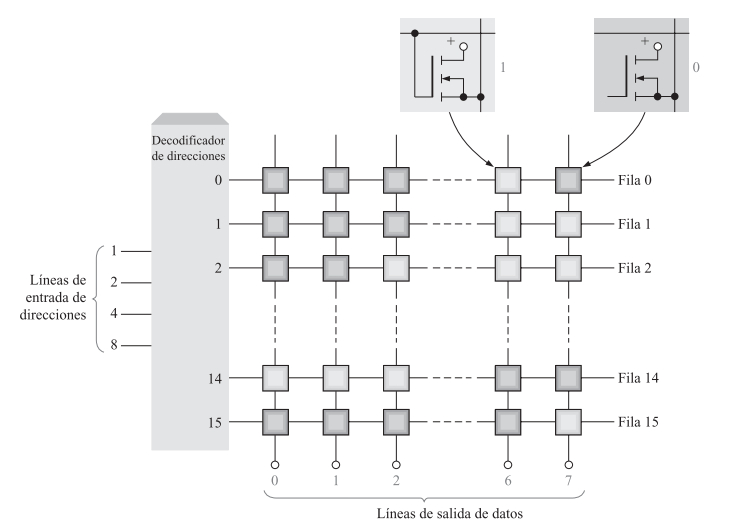
\includegraphics[width=0.7\linewidth]{media/matriz-rom}
		\caption{Representación Matricial de una ROM de 16x8 bits}
		\label{fig:matriz-rom}
	\end{figure}
	
	\subsection{Familias ROM}
	Una memoria ROM se sub-divide en diferentes categorías según la tecnología y método a usar para la escritura o en  caso muy particulares la re-escritura de datos, dentro de esta clasificación, se tiene:
	\begin{itemize}
		\item ROM de máscara
		\item PROM (ROM Programable)
		\item EPROM (ROM Programable Borrable)
		\item UV PROM (ROM Programable Borrrable mediante Rayos Ultravioleta)
		\item EEPROM (ROM Programable Borrable Electricamente)
	\end{itemize}
	
	\subsection{Aplicaciones de la ROM}
	Las ROM son ampliamente utilizadas para el almacenamiento de información de forma no volátil lo que implica que este tipo de memorias no requieren y/o dependen de una fuente de alimentación constante para mantener la información previamente grabada.
	
	\section{Simulación}
	Para poder emular el comportamiento de una memoria ROM se hizo uso del software Quartus en su versión V.20.1 la cual permitió modelar este componentes lógicos mediante el lenguaje de descripción de hardware VHDL.
	
	\begin{figure}
		\centering
		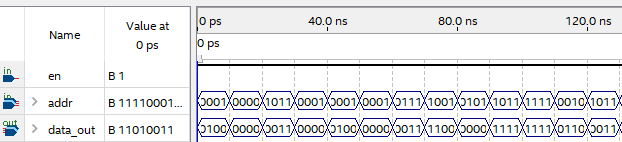
\includegraphics[width=0.7\linewidth]{media/rom8x4-forma-onda}
		\caption{Forma de Onda de salida para la ROM 8x4}
		\label{fig:rom8x4-forma-onda}
	\end{figure}
	
	Como se puede apreciar en le \ref{fig:rom8x4-forma-onda} se puede apreciar que se tiene una salida o lectura de datos en función a una dirección de memoria y su vez esta salida se encuentra en dependencia de la entrada habilitadora que permite el acceso a cada una de las memorias ROM 4x2.
	
	\section{Resultados}
	A lo largo del desarrollo y evolución tecnológica, las memorias ROM han demostrado ser una solución efectiva para el almacenamiento no volátil de datos, donde la información una vez grabada no puede modificarse de forma sencilla siendo necesario para este proceso el uso de procesos específicos.
	
	Las diferentes variantes de la memoria ROM, como la PROM, EPROM, y EEPROM, han permitido que estas memorias se adapten a diversas necesidades tecnológicas, desde el almacenamiento de código fijo en dispositivos electrónicos hasta la posibilidad de reprogramación de estas memoriaas para ciertas aplicaciones.
	
	Finalmente, la simulación de memorias ROM realizada mediante el software Quartus II, utilizando el lenguaje de descripción de hardware VHDL, el cual ha permitido modelar y entender mejor el comportamiento de los módulos ROM, así como su expansión a partir de encapsulados de menor capacidad de palabra o de direcciones.
	
	\section{Recomendaciones}
	\begin{itemize}
		\item La definición VHDL de memorias ROM de gran cantidad de direcciones o tamaño requiere bastante recursos computaciones por lo que es preferible hacer uso de herramientas ya definidas como lo son las librerías de memoria, las cuales optimizan los recursos de hardware.
		\item Para un análisis más complejo y profundo del comportamiento de una ROM se puede tratar este tema desde la perspectiva visual en función a bloques lo cual brinda una mayor comprensión del funcionamiento al realizar las expansiones y definiciones de cada memoria de forma gráfica.
	\end{itemize}
	
	\section{Bibliografía}
	1] Floyd, T. L. (2006). Fundamentos de sistemas digitales (9.ª ed.). Pearson Educación
	
	\newpage
	\section{Anexos}
	\begin{figure}
		\centering
		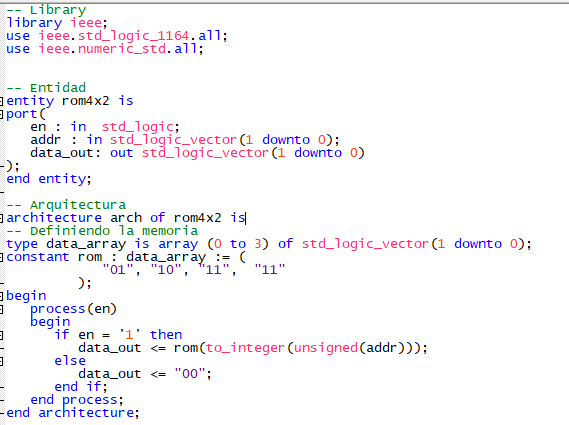
\includegraphics[width=0.7\linewidth]{media/rom4x2}
		\caption{Módulo ROM 4x2}
		\label{fig:rom4x2}
	\end{figure}
	
	\begin{figure}
		\centering
		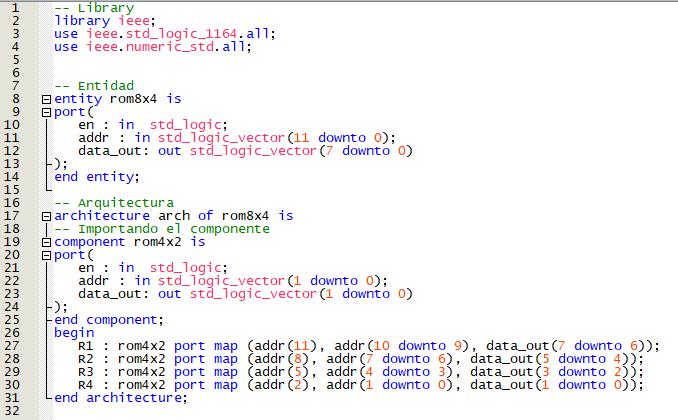
\includegraphics[width=0.7\linewidth]{media/rom8x4}
		\caption{Memoria ROM 8x4 definida de forma estructural}
		\label{fig:rom8x4}
	\end{figure}
	
\end{document}



















